\begin{center}
    \chapter{Datu analīze}
\end{center}

Tā kā no žurnālfailiem ir iegūti dažādi ar GPU izpildi saistītu notikumu
izpildes laiki, kuri starp risinājumiem ir pēc iespējas ielikti ekvivalentās
vietās, tad vienkārši apskatot tekošo kopējo uzkrāto (kumulatīvo) summu,
var vizualizēt katras platformas izpildes laikus pret pietiekami
līdzīgiem atskaites punktiem (skatīt attēlus \ref{img:sha256_100m_not_found_cum},
\ref{img:gol_10k10k_10k_steps_cum}).

\begin{figure}[H]
    \centering
    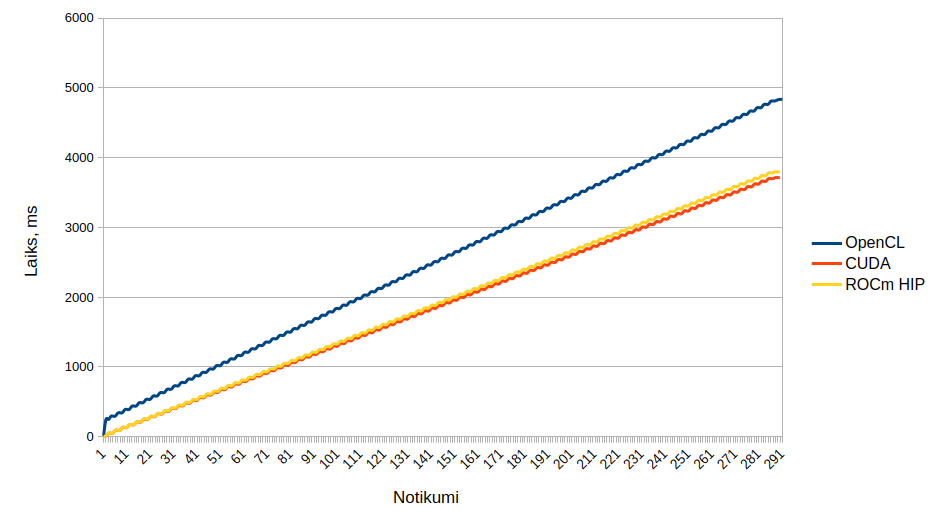
\includegraphics[width=\textwidth]{images/sha256_100m_not_found.png}
    \caption{Paroļu atguvēja izpildes laiki 100m parolēm (parole netika
    atrasta), datu straumes izmērs \( 2^{20} = 1048576\)}
    \label{img:sha256_100m_not_found_cum}
\end{figure}

\begin{figure}[H]
    \centering
    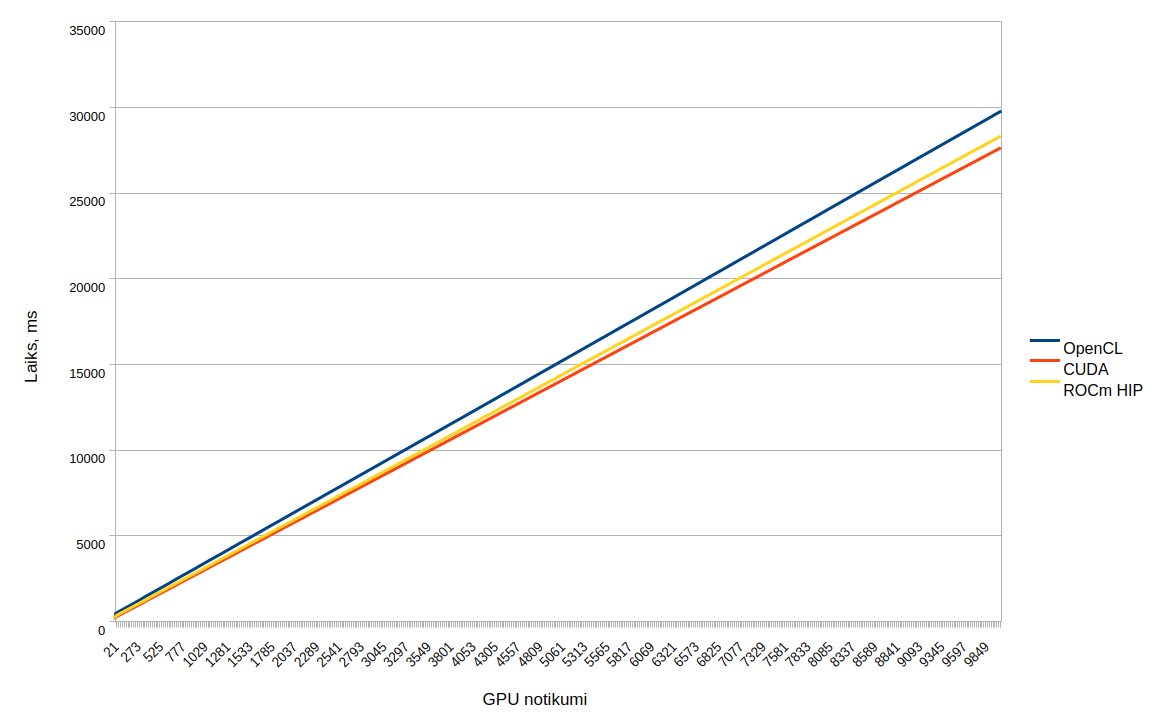
\includegraphics[width=\textwidth]{images/gol_10k_by_10k_10ksteps.png}
    \caption{10000x10000 Dzīves spēle ar 10000 soļiem}
    \label{img:gol_10k10k_10k_steps_cum}
\end{figure}

Pēc grafiem var apstiprināt to, kas jau tika noskaidrots kursa darbā saistībā
ar CUDA un ROCm HIP - ROCm HIP ir neliela virsdarbe, salīdzinot ar
CUDA.\cite{kursa-darbs} Saistībā ar OpenCL platformu, katrs notikums ir,
relatīvi runājot, ar daudz lielāku virsdarbi.

Pēc jaunajiem etalonuzdevumiem var secināt, ka vidēji paroles
atgūšanas uzdevumā OpenCL ir par \(30.18\%\) lēnāks nekā CUDA un Dzīves
spēles uzdevumā par \(7.71\%\) lēnāks. Bet, salīdzinot HIP ar CUDA,
AMD platforma ir par \(2.25\%\) un \(2.47\%\) lēnāka.

Atsevišķi apskatot specifiskus GPGPU notikumus kā kodolu izpilde, starp
platformām varētu atrast kodolu izpildes nestabilitāti, tas ir, izpildes laiki
varētu būt ļoti dažādi, ar lielu variāciju, līdz ar to, ja apskata viena veida
laidienu konfigurāciju starp platformām kā izpildes laiku histogrammu, varētu
noskaidrot cik stabila ir kodolu izpilde.

Tā kā izmantotās videokartes (un CUDA, HIP platformu definētā) notikumu
precizitāte ir līdz \(\pm0.5\)\si{\micro\second}, histogrammas "spaiņa" (angļu
val. \textit{Histogram Bin}) platums noteikts kā \(1\)\si{\micro\second} - nav
pārāk šaura, lai nerastos kļūdas dēļ datu neprecizitātes, un nav pārāk plata, 
ka tiktu zaudēta izšķirtspēja. \cite{Freedman1981} No analizējamajiem datiem
izņemtas pašas pirmās kodolu izpildes programmu dzīves ciklā, kuras var saturēt
inicializācijas un kešatmiņas virsdarbes.

Līdzīgs risinājums izmantots priekš paroļu atguvēja žurnālfailu datiem, ar
papildus datu filtrēšanu, tā lai tiktu iekļautas tās kodolu izpildes, kuras
pilnībā aizņem visu datu straumes buferi, pretēji kodolu izpildes laiki var būt
neparedzami mainīgi.

\begin{figure}[H]
    \centering
    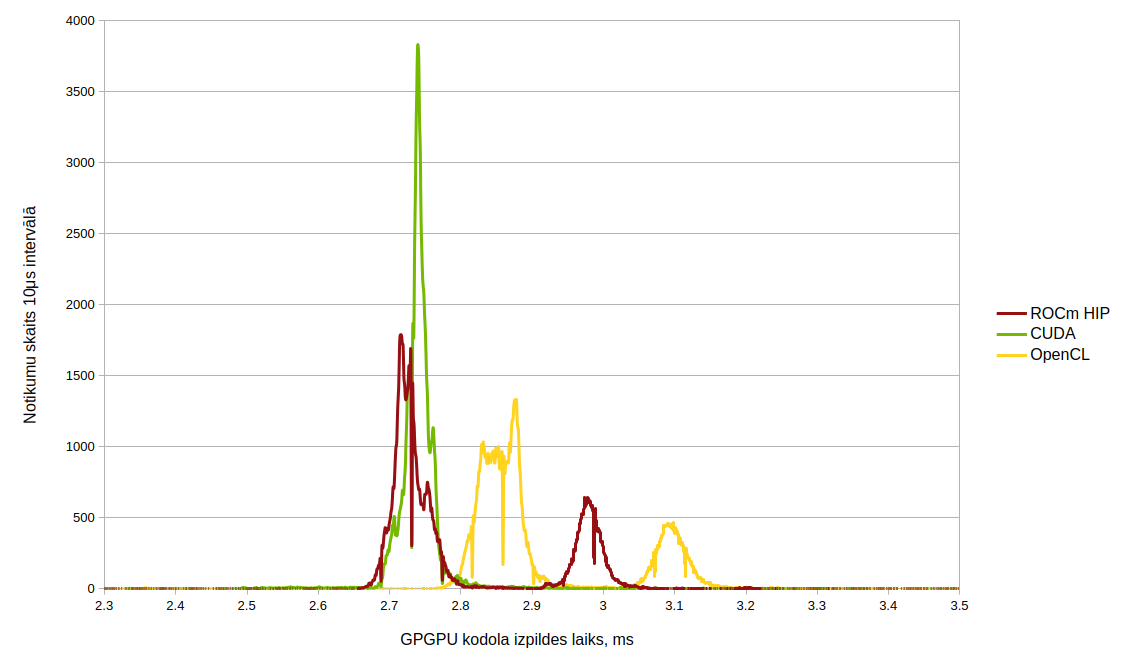
\includegraphics[width=\textwidth]{images/gol_distrib.png}
    \caption{Dzīves spēles kodolu izpildes histogramma (10000x10000 ar 10000 soļiem, 10 laidieni)}
    \label{img:gol_distrib}
\end{figure}


\begin{figure}[H] \centering
    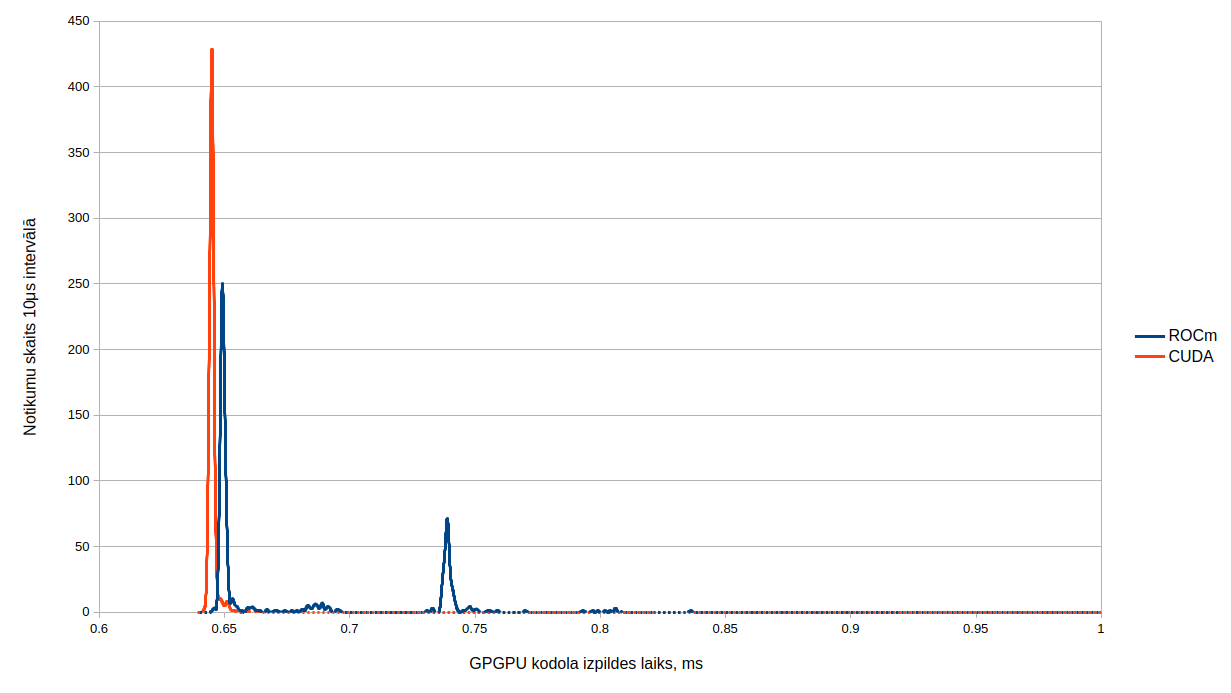
\includegraphics[width=\textwidth]{images/sha_distrib_cuda_rocm.png}
    \caption{Paroļu atguvēja izpildes histogramma CUDA un ROCm platformām (100
    000 000 paroles, 10 laidieni)} \label{img:sha_distrib}
\end{figure}


\begin{figure}[H] \centering
    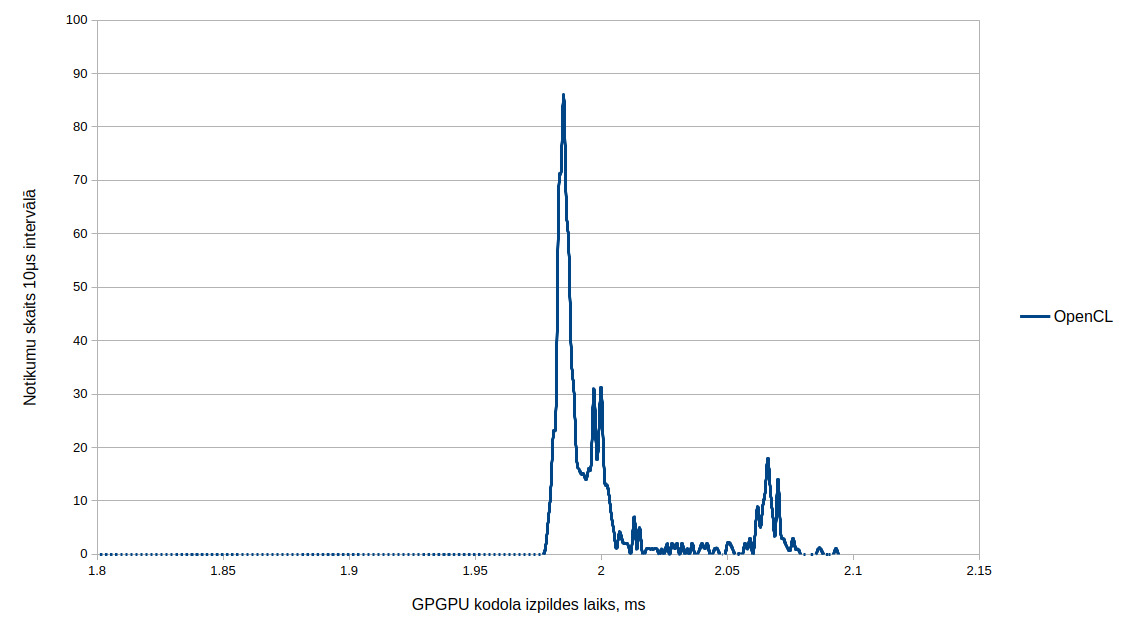
\includegraphics[width=\textwidth]{images/sha_distrib_opencl.png}
    \caption{Paroļu atguvēja izpildes histogramma OpenCL platformai (100 000
    000 paroles, 10 laidieni)} \label{img:sha_distrib_cl}
\end{figure}

Apskatot histogrammu bildes \ref{img:gol_distrib}, \ref{img:sha_distrib},
\ref{img:sha_distrib_cl}, var redzēt, ka mazākā izkliedētība ir CUDA
platformai. Pieņemot, ka datu veido normālo sadalījumu, tabulās \ref{tab:kern},
\ref{tab:kernel_exec_time_variations_gol} redzamas atbilstošās Standartnovirzes
un variācijas.


\begin{table}[H]
    \centering
    \begin{tabular}{lrr}
    \hline
    \textbf{Platforma} & \textbf{Standartnovirze} & \textbf{Variāciju koeficients}\\ \hline
    CUDA    & 0.0015 & 0.0023 \\
    HIP     & 0.0408 & 0.0604  \\
    OpenCL  & 0.0275 & 0.0137 \\
    \hline
    \end{tabular}
    \caption{Platformu paroļu atguvēja kodolu izpildes laiku variācijas}
    \label{tab:kern} 
\end{table}


\begin{table}[H]
    \centering
    \begin{tabular}{lrr}
    \hline
    \textbf{Platforma} & \textbf{Standartnovirze} & \textbf{Variāciju koeficients}\\ \hline
    CUDA    & 0.1613 & 0.0587 \\
    HIP     & 0.1132 & 0.0405  \\
    OpenCL  & 0.1228 & 0.0422 \\
    \hline
    \end{tabular}
    \caption{Platformu Dzīves spēles kodolu izpildes laiku variācijas}
    \label{tab:kernel_exec_time_variations_gol} 
\end{table}


Interesants novērojums ir fakts, ka abos uzdevumu risinājumos, HIP un
OpenCL 


viena kodola izpilde priekš sha un gol pie dažādiem izmēriem





Rezultātu nodaļa!!! Vajag atsevišķā failā

Dažādos griezumos apskatīti iegūti dati no žurnālfailiem.
Kopsummā apstrādāti un analizēti 816 faili par CUDA, HIP, OpenCL
dažādajiem GPGPU notikumu izpildes ilgumiem
